\documentclass[8pt]{beamer}

\mode<presentation>
{
  \usetheme{AnnArbor}
  \usecolortheme{beaver}
  \usefonttheme{default}
  \setbeamertemplate{caption}[numbered]
  \setbeamercovered{transparent}
  \usefonttheme[onlymath]{serif}
  \setbeamertemplate{itemize items}[default]
  \setbeamertemplate{navigation symbols}{\insertslidenavigationsymbol\insertframenavigationsymbol}
} 

\usepackage[english]{babel}
\usepackage[utf8x]{inputenc}
\usepackage{mathtools, xcolor, soul, amsfonts, appendixnumberbeamer, graphicx, tikz, caption}
\usepackage[makeroom]{cancel}
\graphicspath{ {images/} }

%\hypersetup{pdfpagemode=FullScreen}

\title[\scalebox{.8}{Preference Learning Using ANN}]{Preference Learning Using ANN}
\author[\scalebox{.8}{Dariush Hasanpoor}]{Dariush Hasanpoor}
\institute[]{Isfahan University Of Technology}
\date[\scalebox{.8}{Dec. 2015}]{Dec. 2015}

\newcommand{\Xtri}{$\blacktriangleright$ }
\newcommand{\Ytri}{$\triangleright$ }
\newcommand{\itemXtri}{\item[\Xtri]}
\newcommand{\itemYtri}{\item[\Ytri]}
\renewcommand{\|}[1][.3em]{\hspace{#1}|\hspace{#1}}
\renewcommand{\,}[1][.3em]{,\hspace{#1}}
\newcommand\Wider[2][3em]{%
\makebox[\linewidth][c]{\begin{minipage}{\dimexpr\textwidth+#1\relax}\raggedright#2\end{minipage}}}
\newcommand*{\Scale}[2][4]{\scalebox{#1}{$#2$}}%
\DeclarePairedDelimiter\abs{\lvert}{\rvert}%

\makeatletter
    \let\oldabs\abs
    \def\abs{\@ifstar{\oldabs}{\oldabs*}}
\makeatother

\makeatletter
% The following two commands should only be given between frames

% Remove the equation counter from the list of counters that are reset after
% each overlay.
\def\donotresetequations{{%
    \let\@@elt\relax
    \def\@elt##1{%
        \expandafter\ifx\csname ##1\endcsname\c@equation%
        \else%
            \@@elt {##1}%
        \fi%
    }%
    \edef\beamer@overlaycounterresets{\beamer@overlaycounterresets}%
    \let\@elt\relax%
    \def\@@elt{\@elt}%
    \xdef\beamer@overlaycounterresets{\beamer@overlaycounterresets}%
}}

% Add the equation counter from the list of counters that are reset after
% each overlay.
\def\resetequations{\resetcounteronoverlays{equation}}
\makeatother

\newlength{\wideitemsep}
\setlength{\wideitemsep}{\itemsep}
\addtolength{\wideitemsep}{1em}
\let\olditem\item
\renewcommand{\item}{\setlength{\itemsep}{\wideitemsep}\olditem}

\DeclarePairedDelimiter{\ceil}{\lceil}{\rceil}

\definecolor{light-blue}{HTML}{66AFE9}
\definecolor{light-red}{HTML}{F77B7B}
\definecolor{light-green}{HTML}{87D13E}

\newcommand{\subitem}{\item[\Ytri]}
\newcommand{\Cpl}{\emph{Preference Learning} }
\newcommand{\pl}{\emph{preference learning} }
\newcommand{\Cp}{\emph{Preference} }
\newcommand{\p}{\emph{preference} }
\newcommand{\m}[1]{\mathcal{#1}}
\newcommand{\e}[1]{{\emph{#1}}}
\renewcommand{\,}{,\hspace{3pt}}
\renewcommand{\|}{\hspace{3pt}|\hspace{3pt}}
\newcommand{\argmax}{\arg\!\max}
\newcommand{\pr}[2]{{\partial #1 \over \partial #2}}
\renewcommand{\O}{\m{O}}
\newcommand{\outOne}{N_{\succ}}
\newcommand{\outTwo}{N_{\prec}}
\newcommand{\outOneXY}{\outOne([x,y])}
\newcommand{\outTwoXY}{\outTwo([x,y])}
\newcommand{\xy}{x \succ y}
\newcommand{\yx}{y \succ x}

\begin{document}

\donotresetequations

\begin{frame}
  \titlepage
\end{frame}

\begin{frame}{Outline}
  \tableofcontents[hideallsubsections]
\end{frame}

\section{Introduction}
\frame{\tableofcontents[currentsection]}
\subsection{What is preference?}

\begin{frame}{What is preference?}

	\begin{block}{Definition}
	\Cpl refers to the task of learning to predict an order relation on a collection of objects (alternatives).
	\end{block}
    \begin{itemize}
    \item Preference information plays a key role in automated decision making and appears in various guises in AI researches:
    \item[]
        \begin{itemize}
        \subitem Qualitative decision theory
        \subitem Non-monotonic reasoning
        \subitem Constraint satisfaction
        \subitem Planning
        \end{itemize}
    \end{itemize}
\end{frame}

\subsection{Notations}

\begin{frame}{Notations}
	\begin{block}{\textbf{Definition:} \textit{Weak} \Cp}
	A weak \p relation  $\succeq$ on a set $\mathcal{A}$ is a reflexive and transitive binary relation.
	\end{block}
	\begin{block}{\textbf{Definition:} \textit{Strict} \Cp}\center
	$a \succ b  \longleftrightarrow  (a \succeq b) \wedge (b \nsucceq a)$
	\end{block}
    \begin{itemize}
    \item In agreement with preference semantics
        \begin{itemize}
        \item[] \vspace{1em}
            \begin{table}
	            \centering
	            \begin{tabular}{c|l}
	                \textit{Notation} & \textit{Interpretation} \\\hline\rule{0pt}{1.6em}
	                $a \succeq b$ & "alternative $a$ is at least as preferred as alternative $b$." \\\rule{0pt}{1.6em}
	                $a \succ b$ & "alternative $a$ is preferred over alternative $b$."\\
	            \end{tabular}
	        \end{table}
        \end{itemize}
    \end{itemize}
\end{frame}

\subsection{Types of Ranking}

\begin{frame}{Types of Ranking}
    \begin{itemize}
    \setlength\itemsep{1em}
    \item The tasks are categorized as three main problems:\\
        \begin{itemize}
        \subitem \textbf{Label ranking}
        \subitem \textbf{Object ranking}
        \subitem \textbf{Instance ranking}
        \end{itemize}
    \end{itemize}
\end{frame}

\begin{frame}{Types of Ranking}{Object Ranking}
    \begin{block}{\textbf{Task}}\small
    The task of this model is to find a preference ranking order among instances.
    \end{block}
    \vskip .4cm
    \begin{itemize}
    \item[] \textbf{Given}
        \begin{itemize}
        \setlength\itemsep{.5em}
        \subitem A (potentially infinite) set X of objects (each object typically represented by a feature vector).
        \subitem A finite set of pairwise preferences $x_i \succ x_j$, $(x_i , x_j) \in \mathcal{X}\times\mathcal{X}$.
        \end{itemize}
    \item[] \textbf{Find}
        \begin{itemize}
        \setlength\itemsep{1em}
        \subitem A ranking function that, given a set of objects $O \subset X$ as input, returns a permutation(ranking) of these objects.
        \end{itemize}
    \item In the training phase, preference learning algorithms have access to examples for which the order relation is \textbf{(partially)} known.
    \end{itemize}
\end{frame}

\section{Learning To Rank}
\frame{\tableofcontents[currentsection]}

\subsection{Preference Learning With The CmpNN}
\begin{frame}{Preference Learning With The CmpNN}
    \begin{itemize}
    \only<1>{
    \item The method presented in this paper is a pairwise preference learning approach.
    \item The preference function is implemented by a multilayered feed-forward neural network.
    \item A CmpNN has following configurations:
    \item[] \begin{itemize}
    \subitem An input layer with $2d$ units($x\, y \in \mathbb{R}^d$).
    \subitem One hidden layer.
    \subitem An output layer with two units(the “evidence” of the relationships $\xy$ and $\yx$).
    \end{itemize}
    }    
    \only<2>{
    \item Thus, the input to the neural network is the concatenation of the two representations:
    \[[x,y] = [x_1,\ldots,x_d,y_1,\ldots,y_d]\]
    \item The outputs will be denoted by $\outOneXY$ and $\outTwoXY$, respectively, where:
    \item[]
    \begin{itemize}
        \subitem $\outOneXY$ estimates the evidence of $\xy$.
        \subitem $\outTwoXY$ estimates the evidence of $\yx$.
    \end{itemize}
    \item The neural network can be trained with the standard back-propagation algorithm.
    }
    \only<3>{
    \item For each pair of inputs $[x,y]$, the assigned target is:
    \begin{equation}
    t = [t_1\, t_2] = \begin{cases}
    \begin{bmatrix}1 & 0 \end{bmatrix}^T & \xy\\
    \begin{bmatrix}0 & 1 \end{bmatrix}^T & \yx
    \end{cases}
    \end{equation}
    \item The error is measured by the squared error function:
    \begin{equation}
    E([x\, y]\, t) = (t_1 - \outOneXY)^2 + (t_2 - \outTwoXY)^2
    \end{equation}
    \item After training, the model can be used to predict the preference relationship for an input pair of objects $x\, y$ as:
    \begin{equation*}
    \begin{cases}
    \xy & \outOneXY \geq \outTwoXY\\
    \yx & \outOneXY \leq \outTwoXY
    \end{cases}
    \end{equation*}
    }
    \only<4>{
    \item The operators implemented by the preference function, realizes a correct total ordering of the objects only if the following properties hold:
    \item[]
    \begin{enumerate}
    \item \textit{Reflexivity:} both $x \succ x$ and $x \prec x$ hold.
    \item \textit{Equivalence between $\succ$ and $\prec$}: if $\xy$ then $\yx$ and vice versa.
    \item \textit{Anti-symmetry:} if $\xy$ and $\yx$ then $x = y$.
    \item \textit{Transitivity:} if $\xy$ and $y \succ z$, then $x \succ z$ (similarly for the $\prec$ relation).
    \end{enumerate}
    \item The proposed method:
    \item[] \begin{itemize}
        \subitem The reflexivity and the equivalence between $\succ$ and $\prec$ are ensured by the particular architecture adopted for the network.
        \subitem The anti-symmetry property fails only if the two outputs are equal, i.e $\outOneXY = \outTwoXY$ and $x \neq y$ holds. but, since the outputs are real numbers, such an event is very unlikely.
        \subitem The transitivity property is generally hard to be guaranteed by a pairwise preference learning approach and the proposed method does not overcome this limitation.
    \end{itemize}
    }
    \only<5>{
    \item Non-transitive preference functions can still be adopted to sort a set of objects:
    \item[] \begin{itemize}
    \subitem Classical sorting algorithms compare only a small subset of all the possible pairs and return an ordering consistent with those comparisons.
If an algorithm knows, from the comparator response, that $\xy$ and $y \succ z$ hold, then $x \succ z$ is usually assumed without a further comparison.
    % \subitem Even if theoretically an inconsistent comparison operator does not define any total ordering, sorting algorithms automatically chose a consistent subset of the available comparisons in order to define the final ordering.
    \end{itemize}
    }
    \end{itemize}
\end{frame}

\begin{frame}{CmpNN Architecture}
    \only<-3>{\vspace{-2em}
    \begin{figure}
    \centering
    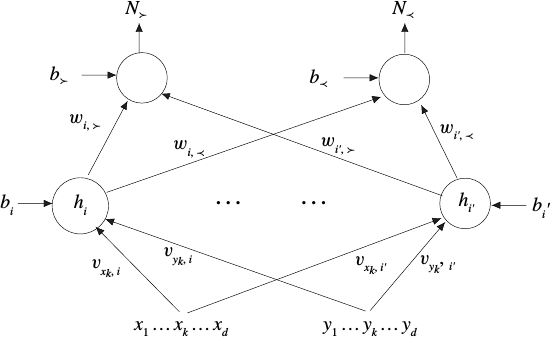
\includegraphics[width=.4\textwidth]{fig1}
    \caption{CmpNN architecture.}
    \end{figure}}
    \begin{itemize}
    \only<1>{\item The CmpNN architecture adopts a weight-sharing technique in order to ensure that the reflexivity and the equivalence between $\succ$ and $\prec$ hold.}
    \only<2>{
    \item Assuming that:
    \item[] \begin{itemize}
        \subitem $\upsilon_{x_k, i}$($\upsilon_{y_k, i}$) denotes the weight of the connection from the input node $x_k$($y_k$) to $i$th hidden node.
        \subitem $w_{i,\succ}$($w_{i,\prec}$) represent the weights of the connections from the $i$th hidden to the output nodes.
    \end{itemize}
    }    
    \only<3>{
    \item For each hidden neuron $i$, a dual neuron $i^\prime$ exists whose weights are shared with $i$ according to the following schema:
    \item[] \begin{enumerate}
    \item $\upsilon_{x_k, i'} = \upsilon_{y_k, i}$ and $\upsilon_{y_k, i'} = \upsilon_{x_k, i}$ hold, i.e., the weights from $x_k\, y_k$ to $i$ are swapped in the connections to $i^\prime$.
    \item $w_{i',\succ} = w_{i,\prec}$ and $w_{i',\prec} = w_{i,\succ}$ hold, i.e., the weights of the connections from the hidden $i$ to the outputs $N_\succ\, N_\prec$ are swapped in the connections leaving from $i'$.
    \item $b_i = b_{i'}$ and $b_\succ = b_\prec$  hold, i.e., the biases are shared between the dual hiddens $i$ and $i'$ and between the outputs $N_\succ$ and $N_\prec$.
    \end{enumerate}
    }
%    \only<4>{
%    \item Why do we have two outputs? Wouldn't it be done by only one output?
%    \item[] \begin{itemize}
%    \subitem There is no a-priori constraint between the values $\outOneXY$ and $\outTwoXY$.
%    \subitem In order to decide which relationship holds for an input pair($[x,y]$), we would need to evaluate also the evidence of the reverse relationship($[y,x]$) -- i.e., $\outOneXY = \outTwoXY$.
%    \subitem In other words, given a pair of objects x and y to be compared, both the $[x,y]$ and $[y,x]$ pairs must be processed by the network to yield the predicted relationship ($\xy$ or $\yx$).
%    \subitem It is equivalent to a CmpNN in which the two values are $\outOneXY$ and $\outTwoXY$ evaluated in two distinct forward phases.
%    \end{itemize}
%    }
    \end{itemize}
\end{frame}

\subsection{LETOR with SortNet}
\begin{frame}{Learning Algorithm}
    \begin{itemize}
    \only<1>{
    \item The CmpNN is embedded into SortNet, as a comparison function.
    %\item In the test phase, the algorithm sorts the objects by calling the CmpNN every time a comparison is needed.
    \item Thus, SortNet can order a set of objects in  $\O(n{\log}n)$.
    }
    \only<2>{
    \item The CmpNN is trained on a dataset, composed of pairs of objects.
    \item The comparative neural network is trained using the square error function that forces the network outputs to be close to the desired targets \underline{on each single pair of objects}.
    %\item When the network produces a perfect classification of any input pair, also the ranking algorithm yields a perfect sorting of the objects.
    \item In general, the optimization of the square error does not necessarily correspond to a good ranking.
    \item A good training procedure should use, in some way, a measure of the quality of the global ordering.
    \item If the number n of the objects is large, then the inclusion of all the $n \choose 2$ pairs into the learning set can make the training very slow or this number of training even may not be useful at all.
    }
    \only<3>{
    \item[] \begin{figure}
    \centering
    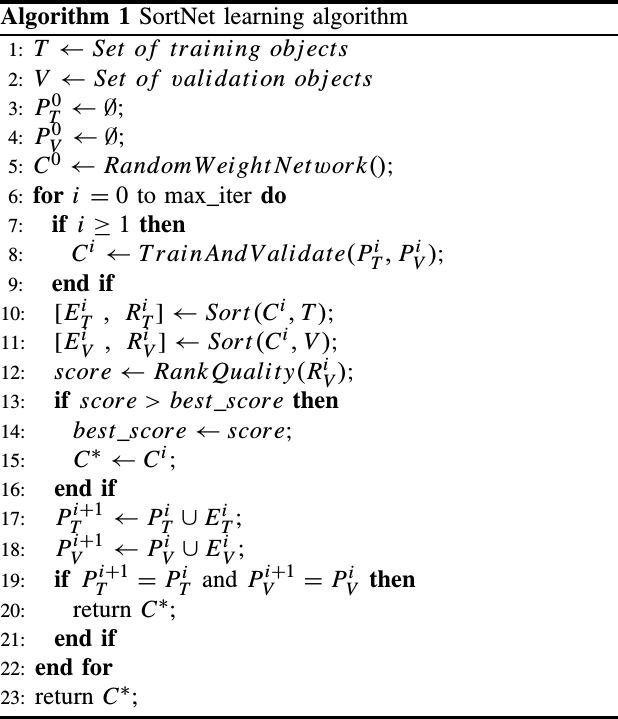
\includegraphics[width=.55\textwidth]{algorithm1}
    \end{figure}
    }
    %\only<4>{
    %\item The idea of building the learning set by choosing the most informative samples from a set of available patterns is basically an \textit{active learning technique}.
    %\item These kind of methods are known also as \textit{Windowing} and they are usually applied for tasks where all the patterns in the learning set are given with their associated targets before starting the training procedure.
    %\item The algorithm can be interpreted as a rough attempt to increase the margin between the mistaken patterns and the separation curve:
    %\item[] \begin{itemize}
    %    \subitem The inclusion of the mis-classified pairs at each iteration is a mechanism by which the learning is focused on the areas of the input domain that are more prone to yield errors.
    %    \subitem On the other hand, the mis-classified patterns are expected to be the closest patterns to the separation curve defined by the classifier.
    %\end{itemize}
    %\item The validation set $P_V$ is in some sense biased because it only contains a subset of the preference pairs. However, preliminary experimental sessions showed that the incremental choice of $P_V$ does not affect the performances significantly.
    %}
    \end{itemize}
\end{frame}

\begin{frame}{Measures of the Ranking Quality}
    \begin{itemize}
%    \only<1>{
%    \item[] \begin{figure}
%    \centering
%    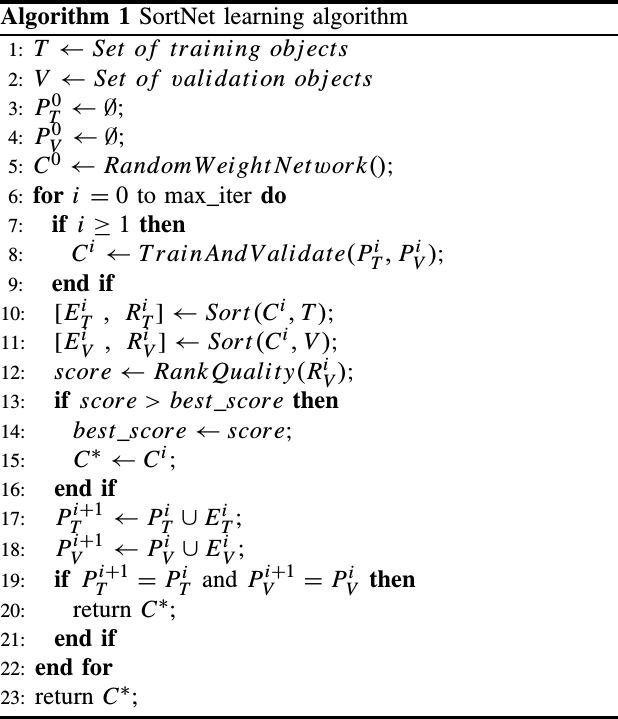
\includegraphics[width=.55\textwidth]{algorithm1}
%    \end{figure}
%    }
    \only<1>{
    \item This paper considered the three measures proposed for the \textit{LETOR} benchmark:
    \item[] \begin{itemize}
    \subitem \textbf{Precision at position n (P@n):} This value measures the relevance of the top n results of the ranking list with respect to a given query:
    \[\text{P@n} = {\text{relevant docs in top n results} \over n}\]
    \subitem \textbf{Mean average precision (MAP):} Given a query $q$, the average precision is:
    \[\text{AP}_q = {\sum_{n = 1}^{N_q} \text{P@n}\cdot \text{rel}(n) \over N_q}\]
    $\text{rel(n)}$ is 1 if the $n$th document in the ordering is relevant and 0 otherwise. Thus, $\text{AP}_q$ averages the values of $\text{P@n}$ over the positions n of the relevant documents.
    \subitem \textbf{Normalized discount cumulative gain (NDCG@n):} This measure exploits an explicit rating of the documents in the list.
    \[\text{NDCG@n} \equiv Z_n\Bigg((2^{r_1} - 1) + \sum_{j = 2}^n{2^{r_j} - 1 \over \log(j)}\Bigg)\]
    where $r_j \geq 0$ is the rating of the $j$th document (smaller values indicate less relevance), and $Z_n$ is a normalization factor chosen such that the ideal ordering gets a $\text{NDCG@n}$ score of 1.
    \end{itemize}
    }
    \end{itemize}
\end{frame}

\subsection{Experimental Results}
\begin{frame}{LATOR Dataset}
    \begin{itemize}
    \only<1>{    
    %\item The SortNet algorithm has been experimentally evaluated on the LETOR datase.
    \item A package of benchmarks for LETOR, released by Microsoft Research Asia and available on the Web.
    \item The task considered in LETOR is that of LETOR, according to their relevance, the documents returned by information retrieval systems in response to a query.
    \item  This paper, considered the version 2.0 of LETOR, which contains three benchmarks:
    \item[] \begin{itemize}
    \subitem \textit{The TD2003 dataset:} consists of 50 sets of documents, each one containing 1000 documents returned in response to a query (i.e., 50 different queries).
    \subitem \textit{The TD2004 dataset:} contains 75 sets of 1000 documents, each corresponding to a different queries.
    \subitem \textit{The OHSUMED dataset:} is a subset of the medical publication repository MEDLINE consists of 106 sets of documents, with associated relevance degrees, that have been returned in response to queries.
    \end{itemize}
    }    
    \only<2>{
    \item For TD2003-2004 datasets:
    \item[] \begin{itemize}
    \subitem Each query-document pair is represented by 44 values that include several features commonly used in information retrieval.
    \subitem A label is assigned to each document to specify whether it is relevant ($\text{R}$) or not ($\text{NR}$) with respect to the given query.
    \subitem For all queries, the relevant documents are roughly 1\% of the whole set of the available documents.
    \end{itemize}
    \item For OHSUMED dataset:
    \item[] \begin{itemize}
    \subitem The relevance degree is provided by humans and consists in one of the following categories: relevant $\text{R}$, possibly relevant $\text{PR}$, and non-relevant $\text{NR}$.
    \subitem The documents are represented using a set of 25 features.
    \end{itemize}
    }
    \end{itemize}
\end{frame}
\begin{frame}{Experimental Results}
    \begin{figure}
    \centering
    \only<1>{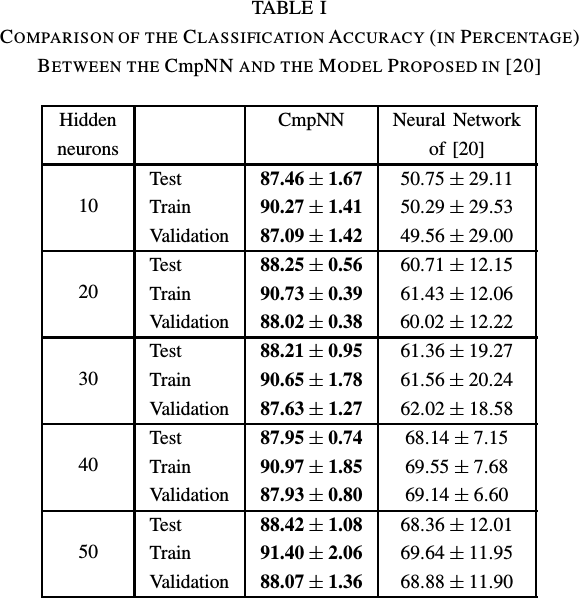
\includegraphics[width=0.4\textwidth]{tab1}}
    %\only<2>{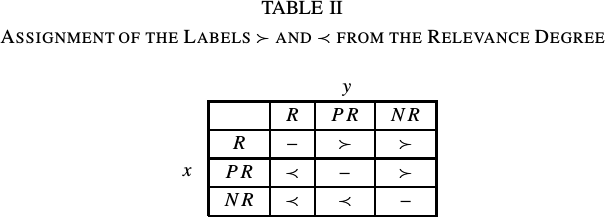
\includegraphics[width=0.5\textwidth]{tab2}}
    \only<2>{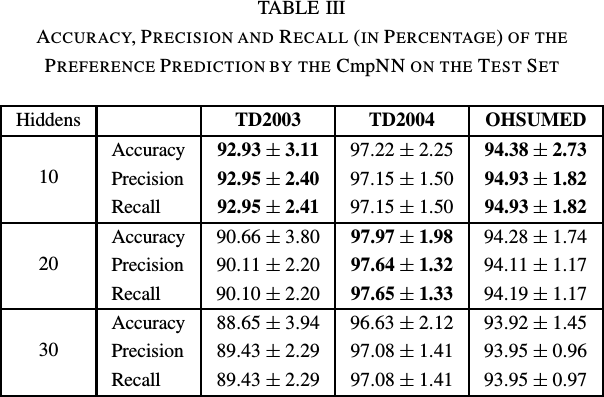
\includegraphics[width=0.5\textwidth]{tab3}}
    \only<3>{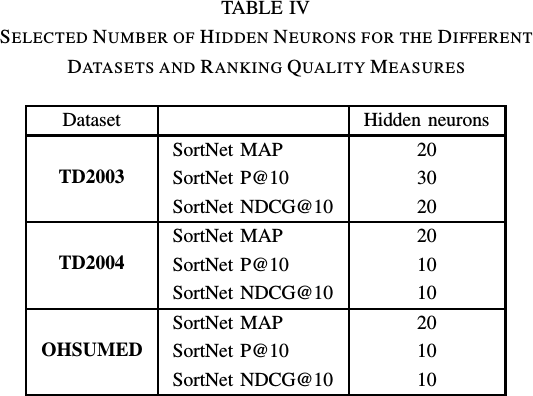
\includegraphics[width=0.5\textwidth]{tab4}}
    \only<4>{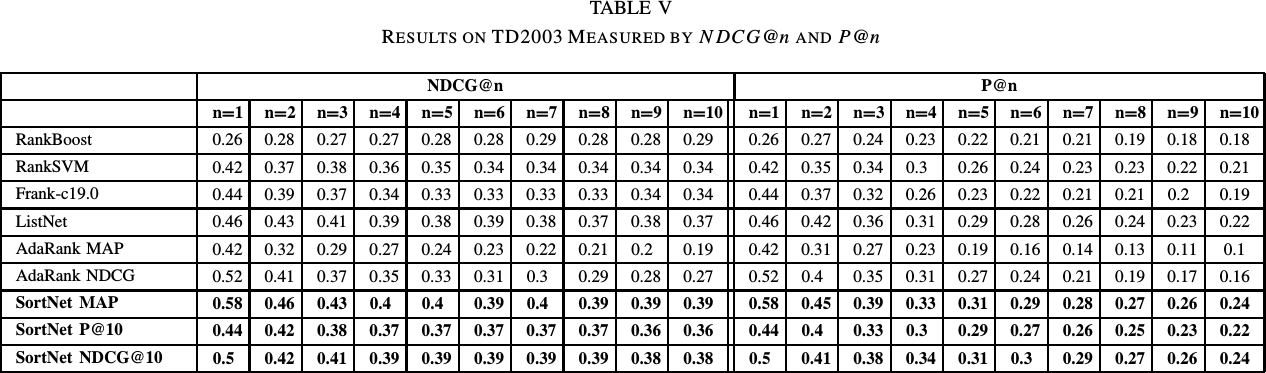
\includegraphics[width=1.0\textwidth]{tab5}}
    \only<5>{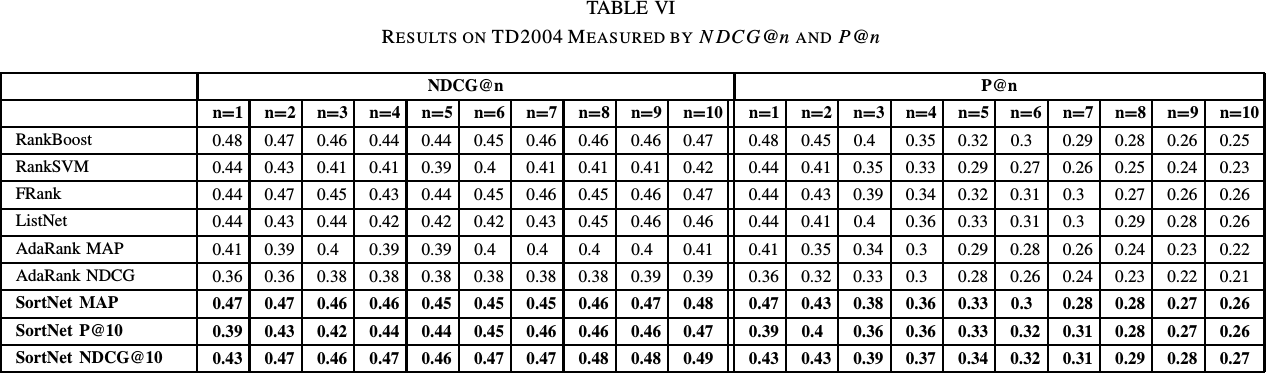
\includegraphics[width=1.0\textwidth]{tab6}}
    \only<6>{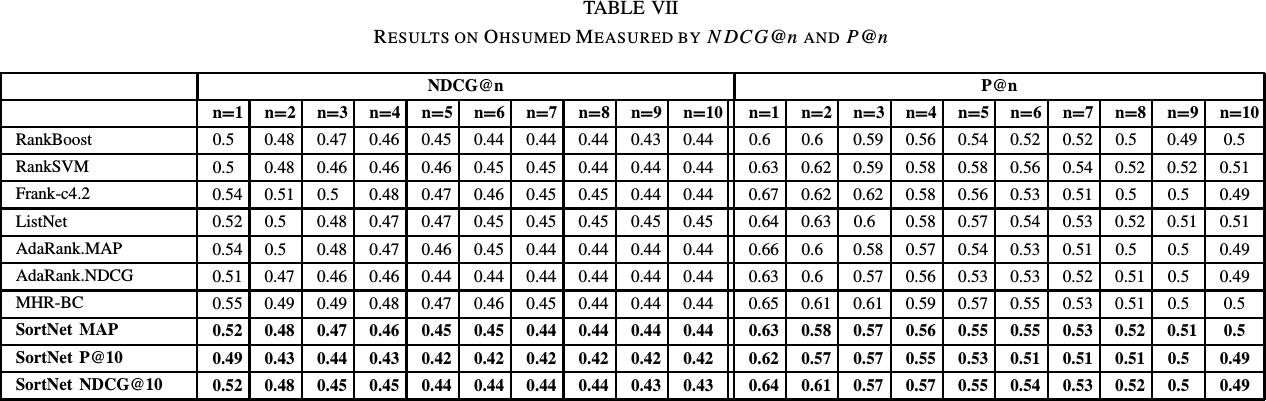
\includegraphics[width=1.0\textwidth]{tab7}}
    \only<7>{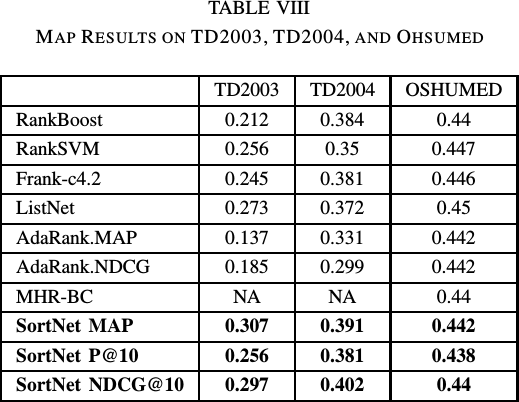
\includegraphics[width=0.5\textwidth]{tab8}}
    %\only<9>{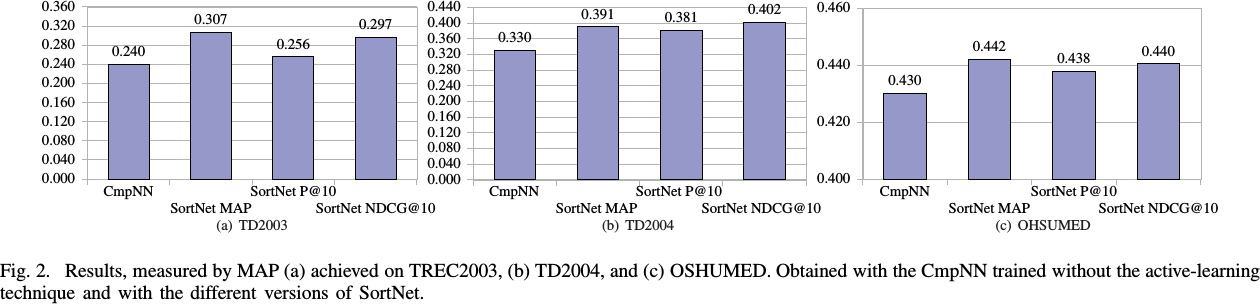
\includegraphics[width=1.0\textwidth]{fig2}}
    %\only<10>{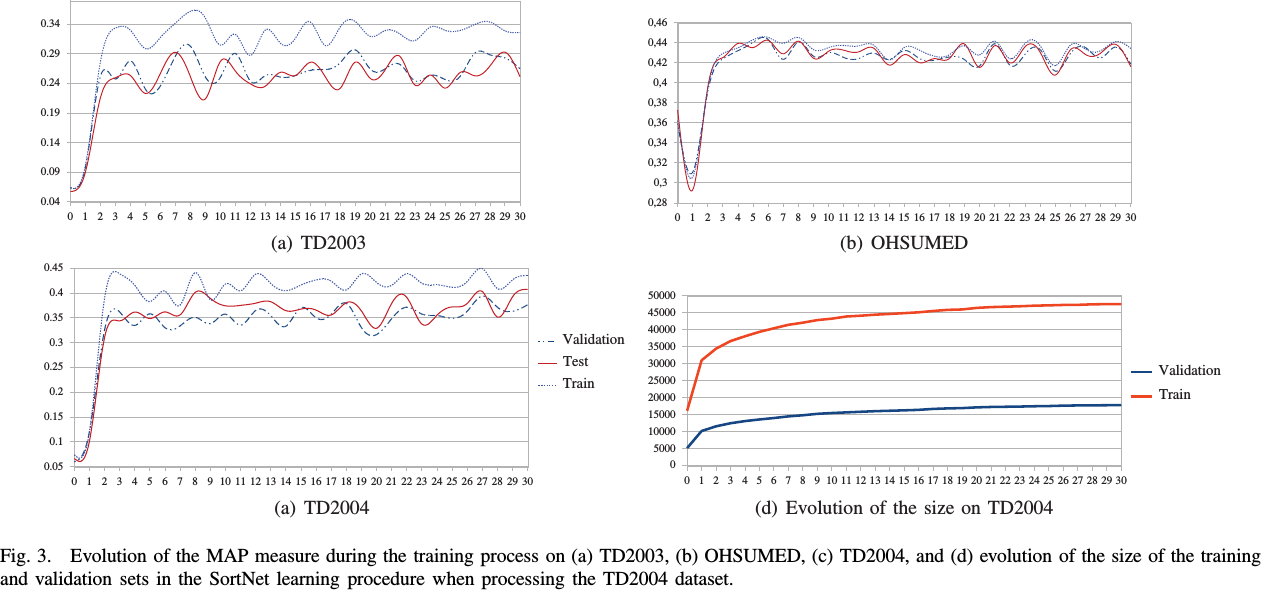
\includegraphics[width=1.0\textwidth]{fig3}}
    %\only<11>{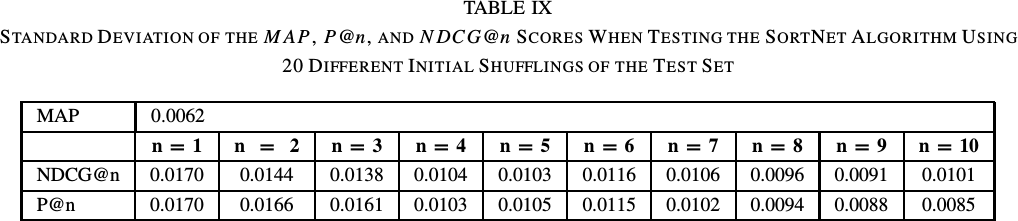
\includegraphics[width=1.0\textwidth]{tab9}}
    %\only<12>{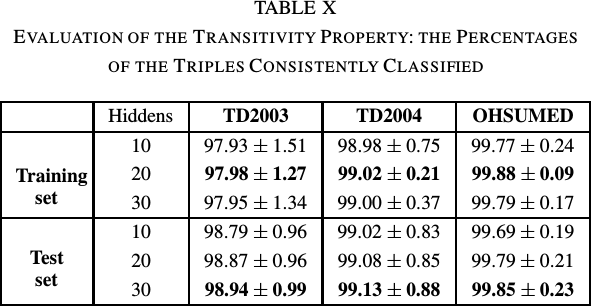
\includegraphics[width=0.5\textwidth]{tab10}}
    \end{figure}
    % the comments about figures
    \begin{itemize}
    \only<1>{\footnotesize
    \item The two models were compared on the task of learning a non–transitive preference function over an artificial dataset. 
    \item The results have been averaged using 5 fold cross validation and for each trial we randomly selected 10,000 pairs for training, 4000 pairs for validation, and 6000 pairs for testing.
    \item The t-student test (with p-value less than 0.05) proves that the model proposed in this paper is able to learn a non-transitive preference function with a significant improvement with respect to the model proposed in [20].
    }
    \only<2>{\item[]}
    \only<3>{\item[]}
    \only<4>{\item[]}
    \only<5>{\item[]}
    \only<6>{\item[]}
    \only<7>{\item[]}
    \end{itemize}
\end{frame}

\section{Conclusion}
\begin{frame}{Conclusion}
    \begin{itemize}
    \item A new neural architecture for learning a preference function (CmpNN) and an adaptive ranking algorithm (SortNet) have been proposed.
    %\item the proposed CmpNN has a particular architecture designed to implement the symmetries naturally present in a preference function.
    \item The SortNet algorithm exploits an iterative procedure aimed at selecting the most informative patterns from the training set. 
    %\item The algorithm has been evaluated using the LETOR datasets, a suite of benchmarks widely used in the LETOR research area.
    \item The results show that the proposed method compares favorably with other state-of-the-art techniques.
    \end{itemize}
\end{frame}

\begin{frame}{}
    \begin{center}
    \vspace{5em}
    {\fontsize{20}{50}\selectfont Thank You!}
    \end{center}
\end{frame}

\section{References}
\begin{frame}{References}
    \nocite{*}
    {\scriptsize
    \bibliographystyle{IEEEtran}
    \bibliography{reference}
    }
\end{frame}

\appendix

\end{document}